\documentclass{article}
\usepackage{graphicx}
\usepackage{appendix}
\usepackage{csvsimple}
\usepackage{amsmath}
\title{Homework 2}
\author{Yuanyou Yao}
\begin{document}
\maketitle{}
\paragraph{Problem 1}
\subparagraph{Method-of-Moments}~{}
\newline
The expectation of uniform distriution is\[E(X)=\frac{\theta}{2}\]
and the first sample moment formula is\[E(X)=\frac{\sum^n_{i=1}x_i}{n}\]
Thus, the method-of-moments estimator of $\theta$ is\[\hat{\theta}=2\frac{\sum^n_{i=1}x_i}{n}\]
\subparagraph{MLE}~{}
\newline
The log-likelyhood function of uniform distribution is\[Ln(\theta)=-nln(\theta)\]
Setting its derivative with respect to parameter $\theta$ to zero, we get:\[\frac{d}{d\theta}lnL(\theta)=\frac{-n}{\theta}\]
which is $< 0$ for $\theta > 0$

Hence, $L(\theta)$ is a decreasing function and it is maximized at $\theta = x_n$, which $x_n$ is the biggest data

The maximum likelihood estimate is thus,\[\hat{\theta}=x_n\]
\subparagraph{Suppose the observations are $x_1=3, x_2=5, x_3=6, x_4=18$}~{}
\newline
According to method-of-moments, the $\hat{\theta}=2\frac{\sum^n_{i=1}x_i}{n}=16$\\
According to MLE, the  $\theta = x_n=18$\\
Obviously, the MLE is better, for MoM of $\theta$ is even smaller than the data, that does make any sense.
\paragraph{Problem2}
\subparagraph{(a)}~{}
\newline
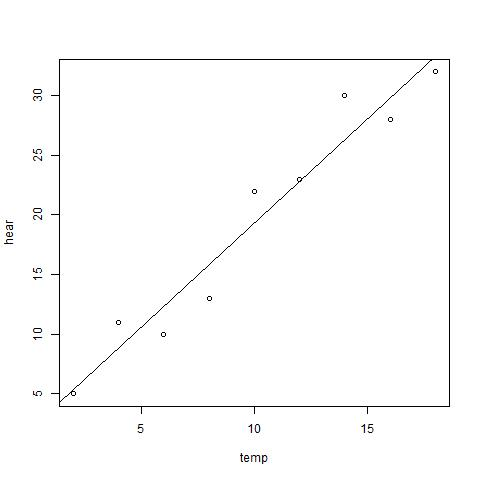
\includegraphics[height=7cm,width=8cm]{2.jpg}

Comment: The graph shows that the two variables are positive correlation, which means while the x becomes larger, y is also becoming larger. The scatters are approximately linear distributed, and the linear regression line looks that it fits the model.
\subparagraph{(b)}~{}
\newline
The linear regrression model is\[Y=1.742X+1.917\]
which the X and Y represent the temperature and heart rate respectively. And the slope1.742 means when X plus 1, Y will add 1.742. The intercept means when then temperature is 0, the heart rate wil be 1.917.
 \subparagraph{(c)}~{}
\newline
Consider the $Y$ $\~$$N(1.742X+1.917,\sigma^2)$\\
we need to calculate the \[\sigma^2=\frac{\Sigma^n_{i=1}e_i^2}{n-2}\] while $n=9, e_i=\hat{Y}-Y$\\
Thus, we have  \[\sigma^2=6.283333\]
So, the underlying population is $Y$ $\~$$N(1.742X+1.917,\sigma^2)$ given the X.
 \subparagraph{(d)}~{}
\newline
Consider the criterion:\[Q=\Sigma^n_{i=1}(Y_i-\beta_0-\beta_1X_i)^2\]
The LS estimators of$\beta_0$ and$\beta_1$ are those values, $\hat{\beta_0}$ and $\hat{\beta}_1 $, that minimize Q, for the given observed data $(X_1,Y_1),...,(X_n,Y_n)$.\\
Differentiate $Q$ with respect to$\beta_0$ and $\beta_1$:\[(a):\frac{\partial{Q}}{\partial{\beta_0}}=-2\Sigma^n_{i=1}(Y_i-\beta_0-\beta_1X_i)\]
\[(b):\frac{\partial{Q}}{\partial{\beta_1}}=-2\Sigma^n_{i=1}(Y_i-\beta_0-\beta_1X_i)X_i\]
Set (a) and (b) equal to 0 and let the solutions to these two
equations be $\beta_0$ and $\beta_1$.\\
By hand calculation, we got the slope is 1.742 and the intercept is 1.917.\\
The slope in the study means when the tempreture goes up 1 C, theheart rate will rise about 1.742. The intercept means when then temperature is 0, the heart rate wil be 1.917.
\subparagraph{(e)}~{}
\newline
At temperature 9 C, estimate the population mean heart rate corresponding to this temperature is $1.742*9+1.917=17.595$. It means that some individuals' heart rate are not exactly 17.595, but the population heart rate at temperature 9 C is 17.595 in average.
\subparagraph{(f)}~{}
\newline
At temperature -2 C, estimate the population mean heart rate corresponding to this temperature is $1.742*(-2)+1.917=-1.567$. However we know that there is no negative heart rate. Although we can predict the dependent variable in mathematical way, it does not make any sense in practice.
\subparagraph{(g)}~{}
\newline
In order to get the population error variance, we then use following estimate method to provide unbaised population error variance:\\
error sum of squares (SSE)\[SSE=\sum_{i=1}^{n}(Y_i-\hat{Y_i})^2=\sum_{i=1}^{n}e^2_i\]
Under simple linear regression, an unbiased estimate of $\sigma^2$ is an error mean square (MSE)\[\hat{\sigma}^2=MSE=\frac{SSE}{n-2}=\frac{\sum_{i=1}^{n}e^2_i}{n-2}\]
Thus, we get\[\hat{\sigma}^2=6.283333\]
Under the assumption of same variance, given the fixed tempreture, the population heart rate variance is 6.283333.
\paragraph{Problem3}
\subparagraph{(a)}~{}
\newline
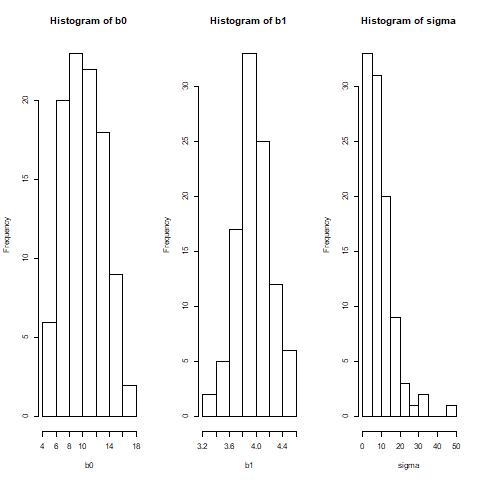
\includegraphics[height=9cm,width=12cm]{31.jpg}
\newline
(i)The intercept $\hat{\beta}_0$ top two frequency is [8,12], which is close to the actual intercept $\beta_0=10$.\\
The slope $\hat{\beta}_1$ top frequency is [3.8,4.0], which is close to the acual slope $\beta_1=4$.\\
The $\hat{\sigma}^2$ top two frequency is [0,10], which is close to the actual $\sigma^2=9$\\
The histogram of the 100  $\hat{\beta}_0$ and $\hat{\beta}_1$ are approximately normal distributed, with their true value most frequent in the histogram. As for the histogram of the 100  $\sigma^2$, the frequency decreases as $\sigma^2$ increases.
(ii)$95\%$
\subparagraph{(b)}~{}
\newline
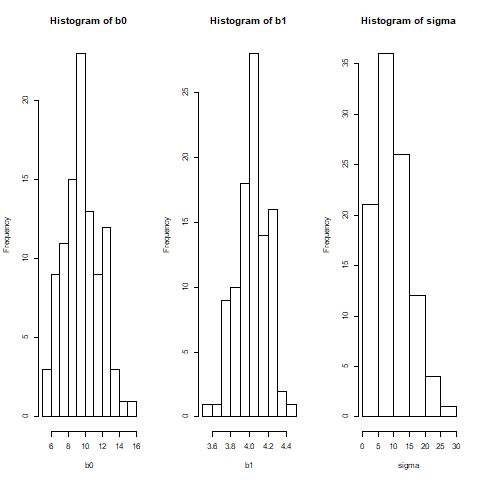
\includegraphics[height=9cm,width=12cm]{32.jpg}
\newline
The histogram of the 100  $\hat{\beta}_0$ and $\hat{\beta}_1$ are aso approximately normal distributed, with their true value most frequent in the histogram. But the variance of them are smaller than in (a). As for the histogram of the 100  $\sigma^2$, the frequency decreases as $\sigma^2$ increases. It reflects the distribution of $\sigma^2$ better, with the highest frequency in the interval [5,10].\\
The proportion of the 100 confidence intervals is 0.96.
\subparagraph{(c)}~{}
\newline
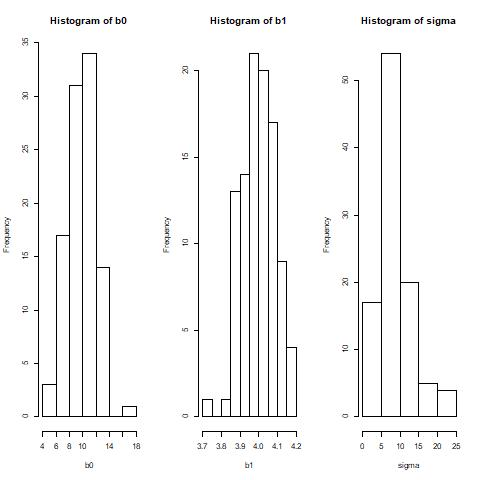
\includegraphics[height=9cm,width=12cm]{33.jpg}
\newline
The histogram of the 100 $\hat{\beta}_0$,$\hat{\beta}_0$ and $\sigma^2$ in (c) are all approximately normal distributed, with their true value most frequent in the histogram. And the variance of them are the smallest among (a), (b) and (c)\\
The proportion of the 100 confidence intervals is 0.95.
\subparagraph{(d)}~{}
\newline
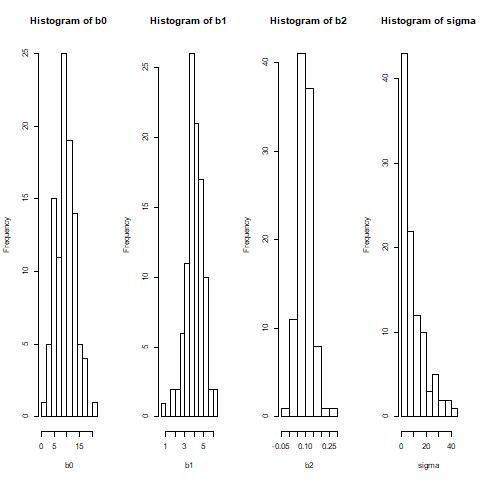
\includegraphics[height=9cm,width=12cm]{34.jpg}
\newline
The distribution of the 100  $\hat{\beta}_0$,$\hat{\beta}_0$ and $\sigma^2$ are similar to (a). But the variance of  $\hat{\beta}_0$,$\hat{\beta}_0$ and $\sigma^2$ in (d) are all bigger than in (a).\\
The proportion of the 100 confidence intervals is 0.97.
\subparagraph{(e)}~{}
\newline
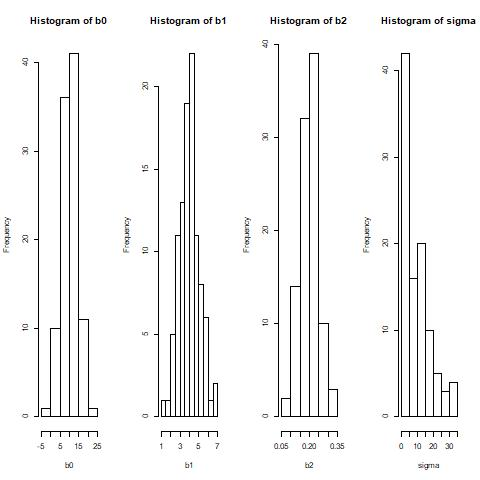
\includegraphics[height=9cm,width=12cm]{35.jpg}
\newline
The distribution of the 100  $\hat{\beta}_0$,$\hat{\beta}_0$ and $\sigma^2$ are similar to (a). But the variance of  $\hat{\beta}_0$,$\hat{\beta}_0$ and $\sigma^2$ in are smaller than in (d) but bigger than in (a).\\
The proportion of the 100 confidence intervals is 0.95.
\section{Problem 4}
\paragraph{(a)}
Under the $H_0$, $\beta_1=0$. The test statistic is: 
$$T=\frac{\hat{\beta}_1-\beta_1}{\sqrt{\frac{\hat{\sigma}^2}{\sum_{i=1}^{n}(x_i-\bar{x})^2}}}\sim T_{n-2},
\ \textup{where} \ \hat{\sigma}^2=\frac{1}{n-2}\sum_{i=1}^{n}(e_i)^2$$
In the frog example, the summary statistic are:\\
$\bar{x}=10,\bar{y}=19.3333,n=9$\\
$s_{xy}=\sum_{i=1}^{n}(x_i-x)(y_i-y)=418,s_{xx}=\sum_{i=1}^{n}(x_i-x)^2=240$\\
$sse=\sum_{i=1}^{n}(y_i-\hat{y})=43.9833,s_{yy}=\sum_{i=1}^{n}(y_i-y)^2=772$\\
The LSE slope and intercept are: $\beta_1=\frac{s_{xy}}{s_{xx}}=1.7417,\\beta_0=\bar{y}-\hat{\beta}_1\times \bar{x}=1.9167$\\
The estimated error variance is: $\hat{\sigma}^2=\frac{sse}{n-2}=6.2833$\\
The estimated standard error of $\hat{\beta}_1$ is: $\hat{se}(\hat{\beta}_1)=\sqrt{\frac{\hat{\sigma}^2}{\sum_{i=1}^{n}(X_i-\bar{X})^2}}=\sqrt{\frac{6.2833}{240}}=0.1618$\\
Thus, the test statistic equals to: $T=\frac{1.7417}{0.1618}=10.7641.$\\
Note that $t_{n-2,\alpha/2}=t_{7,0.025}=2.365<10.7641$. Thus, we can reject $H_0$. A 95\% CI for $\beta_1$ is:
\\ $\hat{\beta}_1\pm t_{n-2,\alpha/2}\times \hat{se}(\hat{\beta}_1)= 1.741 \pm 2.365 \times 0.4281 =[1.3590,2.1243]$.
\paragraph{(b)}
Assume the normality assumption is not valid, then we can employ Bootstrapping to estimate the value of $\beta_1$:
 \begin{itemize}
	\item[1)]
	Firstly, we randomly select 9 observations with replacement from the original dataset and save as dataset $Random(i)$.
	\item[2)]
	Then we fit the simple linear regression model and calculate $\hat{\beta_1}$ based on the random sample, and use $\beta_1^{(i)}$ to denote it.
	\item[3)]
	Repeat 1) and 2) for k times, then we have a vector of $\beta_1^{(1)}, \beta_1^{(2)},...,\beta_1^{(k)}$.
	\item[4)]
	By using the 2.5th and 97.5th percentiles, we can calculate the 95\% empirical interval.
\end{itemize}
Set k = 1000, then we can have the 95\% CI based on Bootstrapping as [1.513127, 2.129650].\\
Compare the result with the 95\% CI calculated from (a), which is [1.3590, 2.1243], we can see the range of the empirical CI is shorter. Besides, the variance for $\hat{\beta_1}$ is 0.1618 and 0.1474316 respectively for (a) and (b). Thus, we can see the empirical CI is a good estimation of $\beta_1$.

\paragraph{(c)}
Since $\sigma=2.5$ is known, 
$$\hat{\beta}_1\sim N(\beta_1,Var(\hat{\beta}_1)),$$
where $Var(\hat{\beta}_1)=\sigma^2(\frac{1}{\sum_{i=1}^{n}(x_i-\bar{x})^2})\approx 0.16^2.$\\
Under the $H_0$: $\beta_1=0$,
$$\hat{\beta_1}|H_0\sim N(0,0.16^2).$$
Rejection region is $|\hat{\beta}_0-0|>1.96\times 0.16.$
Under a particular alternative $H_A:\beta_1=\mu,$
$$\hat{\beta_1}|H_A\sim N(\mu,0.16^2).$$
Power at $\mu$:
$$Power(\mu)=\phi (\frac{\mu}{0.16/\sqrt{9}}-1.96)+\phi (\frac{-\mu}{0.16/\sqrt{9}}-1.96)$$
For $\beta_1=0,\pm 0.5,$ we use the formula above to calculate; for $\beta_1=\pm 1,\pm 1.5,$ we use power.t.test in R to derive results.
Those results are list below:
\begin{table}[]
	\centering
	\begin{tabular}{cccccc}\hline
		$\mu$ & 0 & $\pm 0.5$ & $\pm 1$ & $\pm 1.5$\\ \hline
		$power(\mu)$ & 0.05 & 0.17 & 0.51 & 0.85 \\ \hline
	\end{tabular}
\end{table}

\paragraph{(d)}
 Repeat Bootstrapping but replace with X = 4, 8, 12, 16. Similarly, we follow the steps above:
\begin{itemize}
	\item[1)]
	Firstly, we randomly select 4 observations with replacement from the original dataset and save as dataset $Random(i)$.
	\item[2)]
	Then we fit the simple linear regression model and calculate $\hat{\beta_1}$ based on the random sample, and use $\beta_1^{(i)}$ to denote it.
	\item[3)]
	Repeat 1) and 2) for k times, then we have a vector of $\beta_1^{(1)}, \beta_1^{(2)},...,\beta_1^{(k)}$.
	\item[4)]
	By using the 2.5th and 97.5th percentiles, we can calculate the 95\% empirical interval.
\end{itemize}
Set k = 1000, then we can have the 95\% CI based on Bootstrapping as [0.5, 2.5 ], and the standard deviation for X = 4, 8, 12, 16 is 0.3911133.\\
Then we draw two power curves each for (b) and (c)\\
By comparison, we can see there is a sharp drop for power in Bootstrapping method, while the power curve for SLR model is much smoother.

\paragraph{(e)}
Under the $H_0$:  $\beta_0=0$. The test statistic is: 
$$T=\frac{\hat{\beta}_0-\beta_0}{\hat{\sigma}\sqrt{\frac{1}{n}+\frac{\bar{X}^2}{\sum_{i=1}^{n}(X_i-\bar{X})^2}}}\sim T_{n-2},\
\textup{where}\ \hat{\sigma}^2=\frac{1}{n-2}\sum_{i=1}^{n}e_i^2$$
In the frog example, the estimated standard error of $\hat{\beta_0}$  is:
$$\hat{\sigma}\sqrt{\frac{1}{n}+\frac{\bar{X}^2}{\sum_{i=1}^{n}(X_i-\bar{X})^2}}=6.283333*\sqrt{\frac{1}{9}+\frac{(10)^2}{240}}=1.821045$$
The observed test statistic is:
$$t^*=\frac{\hat{\beta}_0}{\hat{se}(\hat{\beta}_0)}=\frac{1.916667}{1.821045}=1.052509$$
Note that $t_{n-2,\alpha/2}=2.365$. By comparison, the p-value is
$$2\times P(t_{9-2,0.05/2})>0.05$$
That is, we accept $H_0$ at $\alpha=0.05$ level. There is not strong evidence that the heart rate of frog is non-zero for temperature 0 C.\\
A 95\% CI for $\beta_0$ is
$$\beta_0\pm t_{n-2,\alpha/2}\hat{se}(\hat{\beta}_0)=1.916667\pm2.365\times1.821045=[-2.390104,6.223437]$$

\paragraph{(f)}
According to the sampling distribution of SLR estimation, we have:
$$\frac{(n-2)\hat{\sigma}^2}{\sigma^2}\sim \chi_{n-2}^2,\
\textup{where}\ \hat{\sigma}^2=\frac{1}{n-2}\sum_{i=1}^n(Y_i-\hat{Y}_i)^2$$
And this distribution is independent of $\hat{\beta}_0$ and $\hat{\beta}_1$. Thus for $\alpha=0.05$ and $n=9$ we have:
$$P\left\{\chi_{1-\alpha/2}^2(n-2)<\frac{(n-2)}{\sigma^2}\sum_{i=1}^n(Y_i-\hat{Y}_i)^2<\chi_{\alpha/2}^2(n-2)\right\}=1-\alpha$$
That is,
$$P\left\{\frac{(n-2)\sum_{i=1}^n(Y_i-\hat{Y}_i)^2}{\chi_{\alpha/2}^2(n-2)}\leq\sigma^2\leq\frac{(n-2)\sum_{i=1}^n(Y_i-\hat{Y}_i)^2}{\chi_{1-\alpha/2}^2(n-2)}\right\}=1-\alpha$$
Thus, the confidential interval for the error variance $\sigma^2$ under $(1-\alpha)$ significant level is:
$$(\frac{(n-2)\sum_{i=1}^n(Y_i-\hat{Y}_i)^2}{\chi_{\alpha/2}^2(n-2)},\frac{(n-2)\sum_{i=1}^n(Y_i-\hat{Y}_i)^2}{\chi_{1-\alpha/2}^2(n-2)})$$
We set $\alpha=0.05$ and $n=9$, then $\chi_{\alpha/2}^2(n-2)=16.01$,$\chi_{1-\alpha/2}^2(n-2)=1.69$.
\\By hand calculation, we then have 95\% CI for $\sigma^2$ as: [19.23069, 182.17949].

\paragraph{(g)}
 Now we consider the inverse fitted line below 
$$\hat{x}=\frac{1}{\hat{\beta}_1}(y-\hat{\beta}_0)$$
The estimated heart rate at $y_h=9$ is 
$$\hat{\mu}_h=\frac{1}{\hat{\beta}_1}(y_h-\hat{\beta}_0)
=\frac{1}{1.742}(9-1.917)=4.067$$
Note that 
$$\hat{\sigma'}^2=\frac{1}{n-2}\sum_{i=1}^{n}(x_i-\hat{x}_i)^2=2.071$$
The estimated variance of $\hat{\mu}_h$ is 
$$\widehat{Var(\hat{\mu}_h)}=\hat{\sigma'}^2\sqrt{\frac{1}{n}+\frac{(y_h-\bar{y})^2}{s_{yy}}}
=2.071\times(\frac{1}{9}+\frac{(9-19.333)^2}{772})=0.517$$
The 95\% CI for the mean heart rate of temperature at $y_h=9$ is
$$\hat{\mu}_h\pm t_{n-2.\alpha/2}\sqrt{\widehat{Var(\hat{\mu}_h)}}
=4.067 \pm 2.365\times \sqrt{0.517}=[2.367,5.767].$$

\paragraph{(h)}
 In a similar way, the estimated heart rate at $y_h=-2$ is 
$$\hat{\mu'}_h=\frac{1}{\hat{\beta}_1}(y_h-\hat{\beta}_0)
=\frac{1}{1.742}(-2-1.917)=-2.249$$
The estimated variance of $\hat{\mu'}_h$ is 
$$\widehat{Var(\hat{\mu'}_h)}=\hat{\sigma'}^2\sqrt{\frac{1}{n}+\frac{(y_h-\bar{y})^2}{s_{yy}}}
=2.071\times(\frac{1}{9}+\frac{(-2-19.333)^2}{772})=1.451$$
The 95\% CI for the mean heart rate of temperature at $y_h=-2$ is
$$\hat{\mu'}_h\pm t_{n-2.\alpha/2}\sqrt{\widehat{Var(\hat{\mu'}_h)}}
= -2.249\pm 2.365\times \sqrt{1.451}=[-5.0979,0.6003].$$

\paragraph{(i)}
By hand calculation, we have:
$$R^2=1-\frac{\sum_{i=1}^{n}(y_i-\hat{y})^2}{\sum_{i=1}^{n}(y_i-\bar{y})^2}
=1-\frac{\sum_{i=1}^{9}(y_i-\hat{y})^2}{\sum_{i=1}^{9}(y_i-19.333)^2}=0.943$$

\paragraph{(j)}
Sample correlation coefficient:
$$\hat{\rho}=\frac{s_{xy}}{\sqrt{s_{xx}}\sqrt{s_{yy}}}=\frac{418}{\sqrt{240}\sqrt{772}}=0.971$$
Find the Fisher's transformation
$$\lambda(\hat{\rho})=\frac{1}{2}log{\frac{1+\hat{\rho}}{1-\hat{\rho}}}=2.111$$
An 95\% CI for $\lambda(\rho)$ is 
$$\lambda(\rho)\pm z_{0.025}\times \sqrt{\frac{1}{n-3}}=2.111\pm 1.96\times \sqrt{\frac{1}{6}}=[1.311,2.911]$$
Thus, an 95\% CI for $\rho$ is
$$\rho \in [\frac{e^{2\hat{\lambda}_1}-1}{e^{2\hat{\lambda}_1}+1},\frac{e^{2\hat{\lambda}_2}-1}{e^{2\hat{\lambda}_2}+1}]
=[\frac{e^{2\times 1.311}-1}{e^{2\times 1.311}+1},\frac{e^{2\times 2.911}-1}{e^{2\times 2.911}+1}]=[0.865,0.994]$$
Model underlying the inference in this part are listed as below:
\begin{itemize}
	\item Assumption:$x$ and $y$ are from a bivariate normal distribution;
	\item $\lambda(\rho)=\frac{1}{2}log(\frac{1+\rho}{1-\rho})=arctan\ h(\rho)$;
	\item $\lambda(\hat{\rho})=\frac{1}{2}log(\frac{1+\hat{\rho}}{1-\hat{\rho}})\approx N(\lambda(\rho),\frac{1}{n-3})$.
\end{itemize}


\section{Problem 5}

\paragraph{(a)}
 \[Let\ X^*\ denote \ \begin{pmatrix}
1& \frac{X_1}{\sqrt{X_1}}&\\ 
\cdots& \cdots& \\ 
1& \frac{X_n}{\sqrt{X_n}}&
\end{pmatrix} \ \, Y^* \ denote\ (\frac{Y_1}{\sqrt{X_1}},\cdots,\frac{Y_n}{\sqrt{X_n}})'\ and\ \mu_i = \frac{\varepsilon_i}{\sqrt{X_i}} ,\ for\ i= 1,\cdots,n 
\]
In this case, in the new model 
\[Y^*=X^*\beta+\varepsilon ,\ where\ \varepsilon=(\varepsilon_1,\cdots,\varepsilon_n)'\]
We have 
\[Var(\varepsilon_i)=Var(\frac{1}{\sqrt{X_i}}\mu_i)=\frac{1}{X_i}\times Var(\mu_i)=\sigma^2\]
i.e.
\[\varepsilon_1,\cdots,\varepsilon_n \sim i.i.d \ N(0,\sigma^2),\ for\ i= 1,\cdots,n\]
Therefore, we could use ordinary least squares method to estimate $\tilde{\beta}$
\[\tilde \beta=(X^{*'}X^*)^{-1}X^{*'}Y^* \]
In addition,
\[E(\tilde \beta)=(X^{*'}X^*)^{-1}X^{*'}Y^*=\beta\]
\[Var(\tilde \beta)=Var((X^{*'}X^*)^{-1}X^{*'}Y^*)=(X^{*'}X^*)^{-1}X^{*'}(\sigma^2I)X^*(X^{*'}X^*)^{-1}\]
\[=\sigma^2(X^{*'}X^*)^{-1}(X^{*'}X^*)(X^{*'}X^*)^{-1} =\sigma^2(X^{*'}X^*)^{-1}\]
In conclusion, $\tilde \beta \sim N(\beta,\sigma^2(X^{*'}X^*)^{-1}),\ in\ which\ X^*=\begin{pmatrix}
1& \sqrt{X_1}&\\ 
\cdots& \cdots& \\ 
1& \sqrt{X_n}&
\end{pmatrix}$

\paragraph{(b)}
If we use the ordinary least square method despite the weighted variance, we need to find the $\beta$ that minimize 
\[Q(\beta)=(Y-X\beta )^T(Y-X\beta )\]
Set
\[\frac{\partial {Q}(\beta)}{\partial\beta}=0\] 
\[\frac{\partial (Y'Y-2\beta'X'Y+\beta'X'X\beta)}{\partial\beta}=0\]
\[0-2X'Y+2X'X\beta=0\]
Therefore \[\hat \beta=(X'X)^{-1}X'Y\]

\paragraph{(c)}
\subparagraph{1) Distribution of $\hat \beta$}
	\begin{itemize}
	\item [i)] $E(\hat \beta)$
	\[E(\hat \beta)=E((X'X)^{-1}X'Y)=(X'X)^{-1}X'Y=\beta\]
	\item[ii)] $Var(\hat \beta)$
	\[Var(\hat \beta)=Var((X'X)^{-1}X'Y))=(X'X)'X'E(\varepsilon \varepsilon')X(X'X)^{-1}
	\]
	\[=E(\varepsilon \varepsilon')(X'X)^{-1}=\sum_{i=1}^n\sigma_i^2(X'X)^{-1}=\sigma^2\sum_{i=1}^nX_i(X'X)^{-1}\]
	\end{itemize}

In conclusion, $\hat \beta \sim N(\beta,\sigma^2\sum_{i=1}^nX_i(X'X)^{-1} )$

\subparagraph{2) Variance of $\hat{e}$\\}
Raw residual $ \hat{e}=(\hat{e_1},\cdots,\hat{e_n})'=Y-X\hat \beta$\\
Therefore, 
\[Var(\hat{e})=Var(Y-X\hat \beta)=\]

\paragraph{(d)}
\[
Var(\hat \beta)=\sigma^2\sum_{i=1}^nX_i(X'X)^{-1}; \ \ Var(\tilde \beta)=\sigma^2(X^{*'}X^*)^{-1}
\]
Therefore, 
\[Var(\hat \beta)=\sum_{i=1}^nX_i \times Var(\tilde \beta)\]
\newpage
\appendixpage
\paragraph{Problem2}~{}
\newline
temp=c(2,4,6,8,10,12,14,16,18)\\
hear=c(5,11,10,13,22,23,30,28,32)\\
jpeg("2.jpg")\\
plot(temp,hear)\\
a=lm(hear~temp)\\
abline(a)\\
dev.off()\\
sum(a\$residuals $\^$2)/7\\
\paragraph{Problem3}~{}
\newline
X=c(2, 6, 10, 14, 18)\\
n=length(X)\\
e=matrix(nrow = n,ncol=100)\\
Y=matrix(nrow = n,ncol = 100)\\
y=vector()\\
va=vector()\\
b0=vector()\\
b1=vector()\\
CI=matrix(nrow = 2,ncol = 100)\\
sigma=vector()\\
su=0\\
for (i in 1:n) {\\
  su=su+(X[i]-mean(X)) $\^$2}\\
t=qt(0.025,3)\\
for (i in 1:100) {\\
e[,i]=rnorm(n,0,3)\\
Y[,i]=10+4*X+e[,i]\\
b0[i]=summary(lm(Y[,i]~X))\$coefficients[1]
b1[i]=summary(lm(Y[,i]~X))\$coefficients[2]\\
sigma[i]=(summary(lm(Y[,i]~X))\$sigma) $\^$2\\
y[i]=b0[i]+b1[i]*7\\
va[i]=sigma[i]*((1/n)+(7-mean(X)) $\^$2/su)\\
CI[,i]=c(y[i]+t*sqrt(va[i]),y[i]-t*sqrt(va[i]))}\\
jpeg("31.jpg")\\
layout(matrix(c(1,2,3),nrow=1,ncol=3,byrow=T))\\
hist(b0)\\
hist(b1)\\
hist(sigma)\\
dev.off()\\
x=0\\
for (i in 1:100) {\\
  if(38>=CI[1,i]\& 38<=CI[2,i]){x=x+1}}
\end{document}